\chapter{適用例}\label{cha:Indication}
本章では、本研究で提案した手法が正しく動作することを確認する。
適用例として、本提案手法を適用する帳票画像を、図\ref{fig:indication_original}に示す。

\begin{figure}[t]
    \begin{center}
        \fbox{
            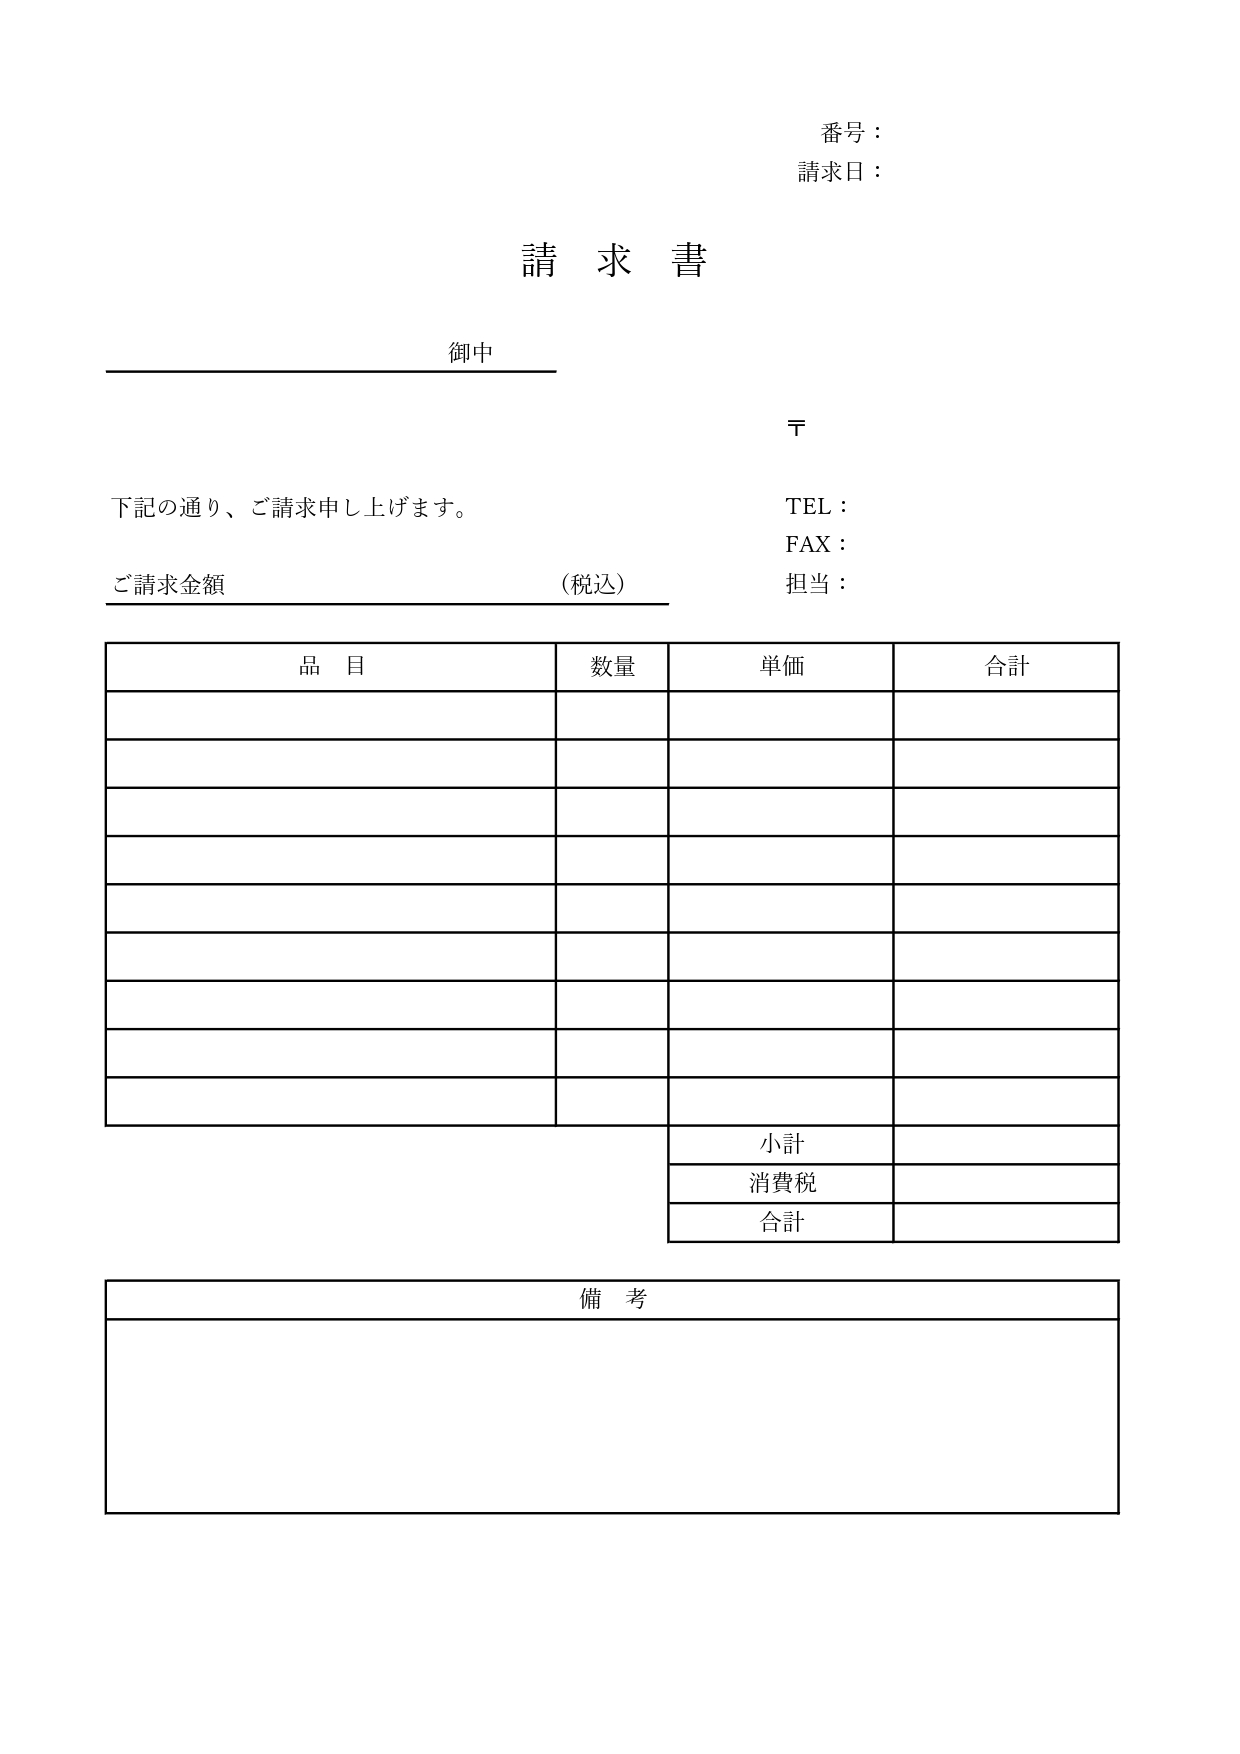
\includegraphics[width=15cm]{image/05-indication/indication_original.jpg}
        }
        \caption{本提案手法を適用する帳票画像}
        \label{fig:indication_original}
    \end{center}
\end{figure}

図\ref{fig:indication_original}に対して、本提案手法を適用し、出力であるJSON形式のファイルと、2枚の領域強調画像を確認する。
具体的には、矩形領域強調画像と、JSON形式のファイルのrects\_data配列を参照し、矩形領域の出力結果を確認する。
同様に、下線部領域強調画像と、JSON形式のファイル内のunderlines\_data配列を参照し、下線部領域の出力結果を確認する。

\section{矩形領域についての出力結果}\label{sec:result_rect}
図\ref{fig:indication_original}に対して、本提案手法を適用し、出力したJSON形式のファイルのうち、rects\_data配列の一部を、図\ref{fig:rects_data_json}に示す。
また、図\ref{fig:rects_data_json}のJSON形式のファイルと同時に出力した2枚の領域強調画像のうち、矩形領域を強調した画像の一部を図\ref{fig:highlighted_rects_part}に示す。

\lstset{language=}
\begin{figure}[t]
    \begin{lstlisting}
        {
            "id": 0,
            "label": "string",
            "coords": {
                "top_left": {
                    "x": 275,
                    "y": 722
                },
                "buttom_left": {
                    "x": 275,
                    "y": 808
                },
                "buttom_right": {
                    "x": 1008,
                    "y": 808
                },
                "top_right": {
                    "x": 1008,
                    "y": 722
                }
            }
        },
        {
            "id": 1,
            "label": "number",
            "coords": {
                "top_left": {
                    "x": 1016,
                    "y": 722
                },
                "buttom_left": {
                    "x": 1016,
                    "y": 808
                },
                "buttom_right": {
                    "x": 1308,
                    "y": 808
                },
                "top_right": {
                    "x": 1308,
                    "y": 722
                }
            }
        },
    \end{lstlisting}
    \caption{rects\_data配列の一部}\label{fig:rects_data_json}
\end{figure}

\begin{figure}[t]
    \begin{center}
        \fbox{
            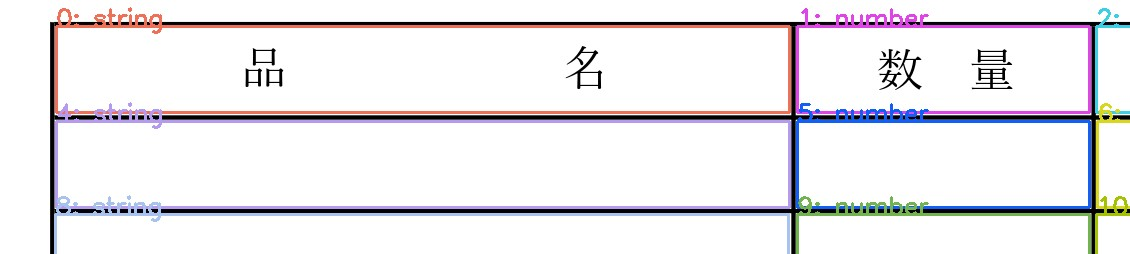
\includegraphics[width=15cm]{image/05-indication/highlighted_rects_part.jpg}
        }
        \caption{矩形領域を強調した画像の一部}
        \label{fig:highlighted_rects_part}
    \end{center}
\end{figure}

図\ref{fig:rects_data_json}より、idキーに対応する値は0、1となっており、それぞれラベルはstring、numberとなっている。
図\ref{fig:highlighted_rects_part}より、画像内に描画した矩形領域の番号のうち、0番と1番の矩形領域には、ラベルをそれぞれstring、numberを割り付けていることがわかる。
これにより、取得した矩形領域については、JSON形式のファイルとPNG形式の矩形領域画像は正しくラベルを割り付けていることが確認できた。


\section{下線部領域についての出力結果}\label{sec:result_underline}
図\ref{fig:indication_original}に対して、本提案手法を適用し、出力したJSON形式のファイルのうち、underline\_data配列の一部を、図\ref{fig:rects_data_json}に示す。
また、図\ref{fig:rects_data_json}のJSON形式のファイルと同時に出力した2枚の下線部強調画像のうち、下線部領域を強調した画像の一部を図\ref{fig:highlighted_rects_part}に示す。

\lstset{language=}
\begin{figure}[t]
    \begin{lstlisting}
        {
            "id": 3,
            "label": "date",
            "left": {
                "x": 868,
                "y": 354
            },
            "right": {
                "x": 1512,
                "y": 354
            }
        },
        {
            "id": 4,
            "label": "string",
            "left": {
                "x": 868,
                "y": 2024
            },
            "right": {
                "x": 1512,
                "y": 2024
            }
        },
        {
            "id": 5,
            "label": "number",
            "left": {
                "x": 1908,
                "y": 354
            },
            "right": {
                "x": 2265,
                "y": 355
            }
        },
    \end{lstlisting}
    \caption{underline\_data配列の一部}\label{fig:underlines_data_json}
\end{figure}

\begin{figure}[t]
    \begin{center}
        \fbox{
            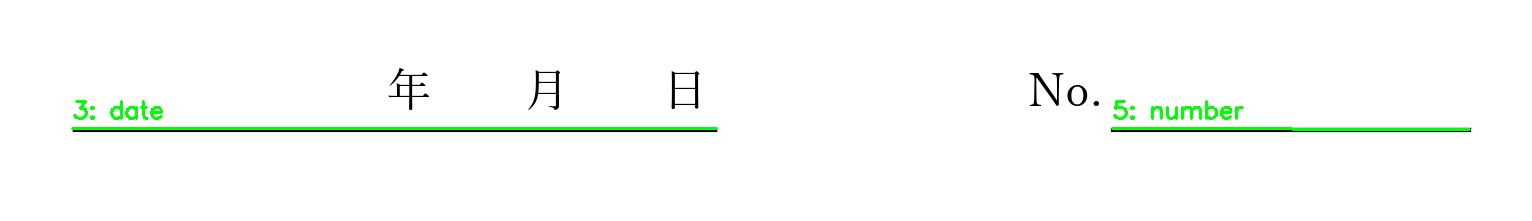
\includegraphics[width=15cm]{image/05-indication/highlighted_underlines_label.jpg}
        }
        \caption{下線部領域を強調した画像の一部}
        \label{fig:highlighted_underlines_part}
    \end{center}
\end{figure}

図\ref{fig:underlines_data_json}のうち、idキーが3、5のオブジェクトに注目する。
図\ref{fig:underlines_data_json}より、idキーに対応する値は3、4、5となっており、それぞれラベルはdate、string、numberとなっている。
図\ref{fig:highlighted_underlines_part}より、画像内に描画した下線部領域の番号のうち、3番と5番の下線部領域には、ラベルをそれぞれdate、numberを割り付けていることがわかる。
これにより、取得した下線部領域については、JSON形式のファイルとPNG形式の下線部領域画像は正しくラベルを割り付けていることが確認できた。